% panqueques
\newpage
%\thispagestyle{empty}
\begin{recipe}[source={La Mami},
portion={12 porciones},
preparationtime={\unit[20]{Minutos}}
]{Panqueques Con Manjar}
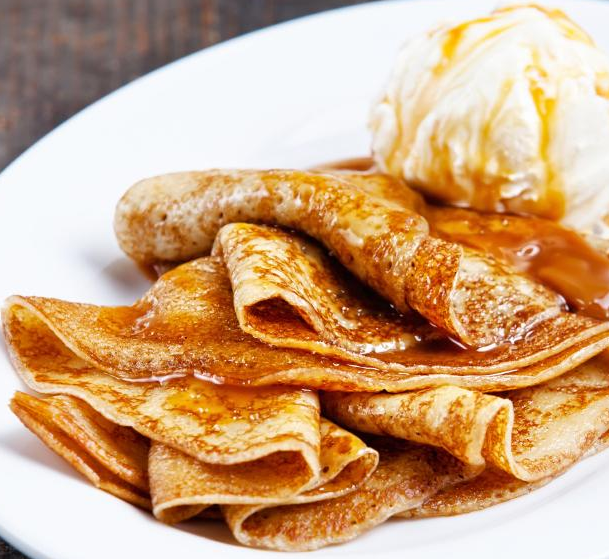
\includegraphics[width=0.25\textwidth]{panqueques}
    \introduction{
        Los panqueques se hacían en casa algunas veces, que buenos recuerdos que me traían de pequeño
        }
    \ingredients{
        1 & Taza y media de leche semidescremada \\
        2 & Huevos \\
        1 & Cucharada de aceite \\
        1 & Taza y media de harina cernida \\
        12 & Cucharadas de manjar \\
    }
    \preparation{
    \begin{enumerate}
            \item Junta todos los ingredientes en el jarro de una juguera vertiendo primero los líquidos como la leche, huevos y aceite y al final los secos (de este modo será más fácil integrar todo), menos el manjar. Procesa a velocidad media durante unos segundos hasta conseguir un batido homogéneo.
            \item Luego calienta una sartén de teflón o antiadherente de diametro mediano, vierte ¾ de un cucharón y distribuye por toda la sartén con movimientos circulares e inclinados con el mango de la sartén. Cocina durante unos segundos hasta dorar sus bordes y voltea. 
            \item Cocina unos segundos mas y repite el procedimiento hasta acabar la mezcla.
            \item Una vez listos, rellénalos uno a uno con una cucharada de manjar  y enróllalos sobre sí mismos, espolvorea azúcar flor y sírvelos de inmediato fríos o calientes como más te guste.
     \end{enumerate}
    }
\end{recipe}